
%% bare_conf.tex
%% V1.4b
%% 2015/08/26
%% by Michael Shell



\documentclass[conference]{IEEEtran}
% Some Computer Society conferences also require the compsoc mode option,
% but others use the standard conference format.
%
% If IEEEtran.cls has not been installed into the LaTeX system files,
% manually specify the path to it like:
% \documentclass[conference]{../sty/IEEEtran}





% Some very useful LaTeX packages include:
% (uncomment the ones you want to load)


% *** MISC UTILITY PACKAGES ***
%
%\usepackage{ifpdf}
% Heiko Oberdiek's ifpdf.sty is very useful if you need conditional
% compilation based on whether the output is pdf or dvi.
% usage:
% \ifpdf
%   % pdf code
% \else
%   % dvi code
% \fi
% The latest version of ifpdf.sty can be obtained from:
% http://www.ctan.org/pkg/ifpdf
% Also, note that IEEEtran.cls V1.7 and later provides a builtin
% \ifCLASSINFOpdf conditional that works the same way.
% When switching from latex to pdflatex and vice-versa, the compiler may
% have to be run twice to clear warning/error messages.








\usepackage{booktabs,chemformula}

\usepackage{graphicx}
\graphicspath{ {images/} }


% *** GRAPHICS RELATED PACKAGES ***
%
%\ifCLASSINFOpdf
%   \usepackage[pdftex]{graphicx}
  % declare the path(s) where your graphic files are
  % \graphicspath{{../pdf/}{../jpeg/}}
  % and their extensions so you won't have to specify these with
  % every instance of \includegraphics
%   \DeclareGraphicsExtensions{.pdf} %,.jpeg,.png}
%\else
  % or other class option (dvipsone, dvipdf, if not using dvips). graphicx
  % will default to the driver specified in the system graphics.cfg if no
  % driver is specified.0
  %\usepackage[dvips]{graphicx}
  % declare the path(s) where your graphic files are
  % \graphicspath{{../eps/}}
  % and their extensions so you won't have to specify these with
  % every instance of \includegraphics
  % \DeclareGraphicsExtensions{.eps}
%\fi
% graphicx was written by David Carlisle and Sebastian Rahtz. It is
% required if you want graphics, photos, etc. graphicx.sty is already
% installed on most LaTeX systems. The latest version and documentation
% can be obtained at: 
% http://www.ctan.org/pkg/graphicx
% Another good source of documentation is "Using Imported Graphics in
% LaTeX2e" by Keith Reckdahl which can be found at:
% http://www.ctan.org/pkg/epslatex
%
% latex, and pdflatex in dvi mode, support graphics in encapsulated
% postscript (.eps) format. pdflatex in pdf mode supports graphics
% in .pdf, .jpeg, .png and .mps (metapost) formats. Users should ensure
% that all non-photo figures use a vector format (.eps, .pdf, .mps) and
% not a bitmapped formats (.jpeg, .png). The IEEE frowns on bitmapped formats
% which can result in "jaggedy"/blurry rendering of lines and letters as
% well as large increases in file sizes.
%
% You can find documentation about the pdfTeX application at:
% http://www.tug.org/applications/pdftex





% *** MATH PACKAGES ***
%
%\usepackage{amsmath}
% A popular package from the American Mathematical Society that provides
% many useful and powerful commands for dealing with mathematics.
%
% Note that the amsmath package sets \interdisplaylinepenalty to 10000
% thus preventing page breaks from occurring within multiline equations. Use:
%\interdisplaylinepenalty=2500
% after loading amsmath to restore such page breaks as IEEEtran.cls normally
% does. amsmath.sty is already installed on most LaTeX systems. The latest
% version and documentation can be obtained at:
% http://www.ctan.org/pkg/amsmath





% *** SPECIALIZED LIST PACKAGES ***
%
%\usepackage{algorithmic}
% algorithmic.sty was written by Peter Williams and Rogerio Brito.
% This package provides an algorithmic environment fo describing algorithms.
% You can use the algorithmic environment in-text or within a figure
% environment to provide for a floating algorithm. Do NOT use the algorithm
% floating environment provided by algorithm.sty (by the same authors) or
% algorithm2e.sty (by Christophe Fiorio) as the IEEE does not use dedicated
% algorithm float types and packages that provide these will not provide
% correct IEEE style captions. The latest version and documentation of
% algorithmic.sty can be obtained at:
% http://www.ctan.org/pkg/algorithms
% Also of interest may be the (relatively newer and more customizable)
% algorithmicx.sty package by Szasz Janos:
% http://www.ctan.org/pkg/algorithmicx




% *** ALIGNMENT PACKAGES ***
%
%\usepackage{array}
% Frank Mittelbach's and David Carlisle's array.sty patches and improves
% the standard LaTeX2e array and tabular environments to provide better
% appearance and additional user controls. As the default LaTeX2e table
% generation code is lacking to the point of almost being broken with
% respect to the quality of the end results, all users are strongly
% advised to use an enhanced (at the very least that provided by array.sty)
% set of table tools. array.sty is already installed on most systems. The
% latest version and documentation can be obtained at:
% http://www.ctan.org/pkg/array


% IEEEtran contains the IEEEeqnarray family of commands that can be used to
% generate multiline equations as well as matrices, tables, etc., of high
% quality.




% *** SUBFIGURE PACKAGES ***
%\ifCLASSOPTIONcompsoc
%  \usepackage[caption=false,font=normalsize,labelfont=sf,textfont=sf]{subfig}
%\else
%  \usepackage[caption=false,font=footnotesize]{subfig}
%\fi
% subfig.sty, written by Steven Douglas Cochran, is the modern replacement
% for subfigure.sty, the latter of which is no longer maintained and is
% incompatible with some LaTeX packages including fixltx2e. However,
% subfig.sty requires and automatically loads Axel Sommerfeldt's caption.sty
% which will override IEEEtran.cls' handling of captions and this will result
% in non-IEEE style figure/table captions. To prevent this problem, be sure
% and invoke subfig.sty's "caption=false" package option (available since
% subfig.sty version 1.3, 2005/06/28) as this is will preserve IEEEtran.cls
% handling of captions.
% Note that the Computer Society format requires a larger sans serif font
% than the serif footnote size font used in traditional IEEE formatting
% and thus the need to invoke different subfig.sty package options depending
% on whether compsoc mode has been enabled.
%
% The latest version and documentation of subfig.sty can be obtained at:
% http://www.ctan.org/pkg/subfig




% *** FLOAT PACKAGES ***
%
%\usepackage{fixltx2e}
% fixltx2e, the successor to the earlier fix2col.sty, was written by
% Frank Mittelbach and David Carlisle. This package corrects a few problems
% in the LaTeX2e kernel, the most notable of which is that in current
% LaTeX2e releases, the ordering of single and double column floats is not
% guaranteed to be preserved. Thus, an unpatched LaTeX2e can allow a
% single column figure to be placed prior to an earlier double column
% figure.
% Be aware that LaTeX2e kernels dated 2015 and later have fixltx2e.sty's
% corrections already built into the system in which case a warning will
% be issued if an attempt is made to load fixltx2e.sty as it is no longer
% needed.
% The latest version and documentation can be found at:
% http://www.ctan.org/pkg/fixltx2e


%\usepackage{stfloats}
% stfloats.sty was written by Sigitas Tolusis. This package gives LaTeX2e
% the ability to do double column floats at the bottom of the page as well
% as the top. (e.g., "\begin{figure*}[!b]" is not normally possible in
% LaTeX2e). It also provides a command:
%\fnbelowfloat
% to enable the placement of footnotes below bottom floats (the standard
% LaTeX2e kernel puts them above bottom floats). This is an invasive package
% which rewrites many portions of the LaTeX2e float routines. It may not work
% with other packages that modify the LaTeX2e float routines. The latest
% version and documentation can be obtained at:
% http://www.ctan.org/pkg/stfloats
% Do not use the stfloats baselinefloat ability as the IEEE does not allow
% \baselineskip to stretch. Authors submitting work to the IEEE should note
% that the IEEE rarely uses double column equations and that authors should try
% to avoid such use. Do not be tempted to use the cuted.sty or midfloat.sty
% packages (also by Sigitas Tolusis) as the IEEE does not format its papers in
% such ways.
% Do not attempt to use stfloats with fixltx2e as they are incompatible.
% Instead, use Morten Hogholm'a dblfloatfix which combines the attributes
% of both fixltx2e and stfloats:
%
% \usepackage{dblfloatfix}
% The latest version can be found at:
% http://www.ctan.org/pkg/dblfloatfix




% *** PDF, URL AND HYPERLINK PACKAGES ***
%
%\usepackage{url}
% url.sty was written by Donald Arseneau. It provides better support for
% handling and breaking URLs. url.sty is already installed on most LaTeX
% systems. The latest version and documentation can be obtained at:
% http://www.ctan.org/pkg/url
% Basically, \url{my_url_here}.




% *** Do not adjust lengths that control margins, column widths, etc. ***
% *** Do not use packages that alter fonts (such as pslatex).         ***
% There should be no need to do such things with IEEEtran.cls V1.6 and later.
% (Unless specifically asked to do so by the journal or conference you plan
% to submit to, of course. )


%\usepackage[table]{xcolor}

% correct bad hyphenation here
\hyphenation{op-tical net-works semi-conduc-tor}


\begin{document}
%
% paper title
% Titles are generally capitalized except for words such as a, an, and, as,
% at, but, by, for, in, nor, of, on, or, the, to and up, which are usually
% not capitalized unless they are the first or last word of the title.
% Linebreaks \\ can be used within to get better formatting as desired.
% Do not put math or special symbols in the title.
%\title{Investigating class attributes in the context of ranking classes according to their importance in object oriented systems }

%\title{What makes class co-changes into logical dependencies ?}
\title{Logical dependencies between classes: how to find them and how to use them ?}


\author{\IEEEauthorblockN{Adelina Diana Stana \\ student - early pre-doctoral track}
\IEEEauthorblockA{Department of Computer and Information Technology, \\ Politehnica University of Timisoara, Romania }
\and
\IEEEauthorblockN{Ioana \c{S}ora and Vladimir Cre\c{t}u\\ supervisors}
\IEEEauthorblockA{Department of Computer and Information Technology, \\ Politehnica University of Timisoara, Romania }

}






% use for special paper notices
%\IEEEspecialpapernotice{(Invited Paper)}




% make the title area
\maketitle

% As a general rule, do not put math, special symbols or citations
% in the abstract
\begin{abstract}

Emerging software engineering approaches support the idea that general methods and tools for dependency management should take into account not only structural dependencies but also logical dependencies. In this work we try to identify a set of factors that can be used to filter the recordings of class co-changes such that true logical dependencies are identified. Also we analyze the impact of filtering factors over the relationships between the sets of logical and structural dependencies and their intersection and differences. We present preliminary results obtained through an experimental study on a set of open source software projects with their historical evolution, and outline additional factors which need to be investigated in future work.

\end{abstract}

% no keywords



\section{Introduction}
\label{sec:intro}
The current trend recommends \cite{Oliva:2011:ISL:2067853.2068086}, \cite{DBLP:journals/jss/AjienkaC17}, \cite{Yu2007} that general dependency management methods and tools should also include logical dependencies besides the structural dependencies that are extracted by analyzing the source code. Gall \cite{Gall:1998:DLC:850947.853338} identified as logical coupling between two modules the fact that these modules repeatedly change together during the historical evolution of the software system.

The concepts of logical coupling and logical dependencies were first used in different analysis tasks, all related to changes: for software change impact analysis \cite{1553643}, for identifying the potential ripple effects caused by software changes during software maintenance and evolution \cite{DBLP:conf/issre/OlivaG15}, \cite{Oliva:2011:ISL:2067853.2068086}, \cite{Poshyvanyk2009}, \cite{posh2010} or for their link to deffects \cite{wiese}, \cite{Zimmermann:2004:MVH:998675.999460}. But, in order to add logical dependencies besides structural dependencies as inputs for methods and tools for dependency management and analysis, class co-changes must be filtered until they remain only a reduced but relevant set of true logical dependencies. 

\section{Research questions}
\label{sec:question}

We investigated through three questions \cite{mastersthesis}, \cite{SoftwareMining2018} the factors that could be used to filter logical dependencies:


\textit{\textbf{Question 1}}. How does the maximum number of source files accepted to change in a commit influence the logical dependencies of the system ? 

\textit{Motivation}: A commit that has as participants a big number of files can indicate that a merge with another branch or a folder renaming has been made. In this case, a series of irrelevant logical dependencies can be introduced since not all the files are updated in the same time for a development reason. Different works have chosen fixed threshold values for the number of files accepted in a commit: \cite{DBLP:journals/jss/AjienkaC17}, \cite{DBLP:journals/ese/AjienkaCC18}, \cite{Beck:2011:CMC:2025113.2025162}.



\textit{\textbf{Question 2}}. Considering changes in comments only as valid can lead to additional logical dependencies?

\textit{Motivation}: We consider that there is probably no logical dependency between two classes that change in the same time only by comments changes. Some studies have not considered this aspect, so we will analyse the impact of considering/not considering changes in comments as valid logical dependencies.

\textit{\textbf{Question 3}}. How many occurrences of a logical dependency are needed to consider it a \textit{valid} logical dependency ? 

\textit{Motivation}: One occurrence of a logical dependency between two classes can be a valid logical dependency, but can also be a coincidence. On the other hand, if the project studied has a relatively small amount of commits, the probability to find multiple updates of the same classes in the same time can be small, so filtering after the number of occurrences can lead to filtering all the logical dependencies extracted. 

\section{Tool for measuring software dependencies}
\label{sec:tool}

\begin{figure*}[htb]
\centering
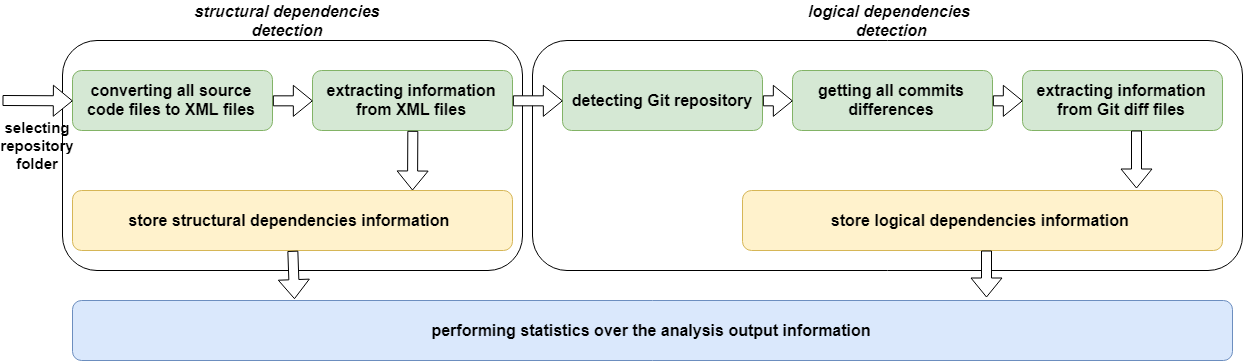
\includegraphics[width=\textwidth]{fig3.png}
\caption{Processing phases}
\label{fig:fig3}
\end{figure*}

In order to build structural and logical dependencies we have developed a tool that takes as input the source code repository and builds the required software dependencies. The workflow of the tool is presented in Figure \ref{fig:fig3}.




\subsection{ Extracting structural dependencies}

A structural dependency between two classes A and B is given by the fact that A statically depends on B, meaning that A cannot be compiled without knowing about B. In object oriented system, this dependency can be given by many types of relationships between the two classes: A extends B, A implements B, A has attributes of type B, A has methods which have type B in their signature, A uses local variables of type B.


 We use an external tool called srcML \cite{2003:XLC:851042.857028}, \cite{Collard:2011:LTF:2067850.2068011} to convert all source code files from the current release into XMl files. All the information about classes, methods, calls to other classes are afterwards extracted by our tool parsing the XML files and building a dependencies data structure. We have chosen to rely on srcML as a preprocessing tool because it reduces a significant number of syntactic differences from different programming languages and can make easyer the parsing of source code written in different programming languages such as Java, C++ and C\#.    

\subsection{Extracting logical dependencies}

The versioning system contains the long-term change history of every file. Each project change made by an individual at a certain point of time is contained into a commit \cite{svn}, \cite{DBLP:journals/jss/AjienkaC17}. 

The tool looks through the main branch of the project and gets all the existing commits. For each commit a diff against the parent commit is made and stored. Here we have the option to ignore commits that contain more files than a threshold value for commit size. Also, we have the option to check whether the differences are in actual code or if they affect only parts of source files that are only comments.  Finally after all the difference files are stored, all the files are parsed and logical dependencies are build. For a group of files that are committed together, logical dependencies are added between all pairs formed by members of the group. Adding a logical dependency increases a occurrence counter for the logical link. 

\section{Experimental results}
\label{sec:experiments}


We have analysed a set of open-source projects found on GitHub\footnote{http://github.com/} in order to extract the structural and logical dependencies between classes \cite{Kalliamvakou2016}. Table \ref{table:1} enumerates all the systems studied.

\begin{table}[h]
	\caption{Summary of open source projects studied.}
	\centering
  \begin{tabular}{@{}ccccc@{}}
    \toprule
    ID  & Project    & Nr. of classes & Nr. of commits& Type\\
    \midrule
 \ch{1}	&	urSQL	&	39	&	89	&	java	\\
 \ch{2}	&	prettyfaces	&	257	&	207	&	java	\\
 \ch{3}	&	jbal	&	102	&	113	&	java	\\
\ch{4}	&	guavatools	&	209	&	85	&	java	\\
\ch{5}	&	monome-pages	&	196	&	280	&	java	\\
\ch{6}	&	kryo	&	289	&	743	&	java	\\
\ch{7}	&	slema	&	267	&	368	&	java	\\
\ch{8}	&	bluecove	&	386	&	1679	&	java	\\
\ch{9}	&	aima-java	&	818	&	1181	&	java	\\
\ch{10}	&	powermock	&	803	&	1512	&	java	\\
\ch{11}	&	restfb	&	713	&	1545	&	java	\\
\ch{12}	&	rxjava	&	2251	&	2468	&	java	\\
\ch{13}	&	metro-jax-ws	&	365	&	2222	&	java	\\
\ch{14}	&	mockito	&	1121	&	1572	&	java	\\
\ch{15}	&	grizzly	&	1170	&	3122	&	java	\\
\ch{16}	&	shipkit	&	222	&	1483	&	java	\\
\ch{17}	&	Tensorflow	&	1104	&	2386	&	cpp	\\

    \bottomrule
  \end{tabular}
  
   \label{table:1}
\end{table}

For each system, we extracted its structural dependencies, its logical dependencies and determined the overlap between the two dependencies sets, in various experimental conditions. 

One variable experimental condition is whether changes in comments only count as logical dependencies: 
\begin{itemize}
	\item with comments: a change in source code files is counted towards a logical dependency, even if the change is only inside comments 
	\item without comments: commits that changed source code files only by editing comments are ignored as logical dependencies
\end{itemize}

In all cases, we varied the following threshold values: 
 \begin{itemize}
	\item commit size ($cs$): the maximum number of files allowed in a commit to be counted as logical dependency. The values for this threshold were 5, 10, 20 and no threshold (infinity).  
	\item number of occurrences ($occ$): the minimum number of repeated occurrences for a co-change to be counted as logical dependency. The values for this threshold were 1, 2, 3 and 4.  
\end{itemize}



\begin{table}[!h]
%% increase table row spacing, adjust to taste
\renewcommand{\arraystretch}{1.10}
\caption{Median values obtained for experiments done}
\label{tab:perc}
\centering

\begin{tabular}{|c|c|c|c|c|}
\hline
	      &	$cs\leq 5$	&	$cs\leq 10$	&	$cs\leq 20$	&	$cs< \infty$	\\
\hline
\multicolumn{5}{c}{A. Percentage of SD that are also LD, case with comments}\\
\hline
$occ\geq 1$	&	13.77	&	23.27	&	36.04	&	66.48	\\
$occ\geq 2$	&	4.11	&	9.90	&	15.79	&	42.05	\\
$occ\geq 3$	&	1.92	&	5.82	&	8.41	&	21.15	\\
$occ\geq 4$	&	0.85	&	2.68	&	5.80	&	13.46	\\
\hline
\multicolumn{5}{c}{B. Percentage of SD that are also LD, case without comments}\\
\hline
$occ\geq 1$	&	13.77	&	22.15	&	34.38	&	63.96	\\
$occ\geq 2$	&	3.67	&	9.17	&	12.53	&	34.62	\\
$occ\geq 3$	&	1.82	&	4.03	&	6.83	&	17.60	\\
$occ\geq 4$	&	0.67	&	2.34	&	4.47	&	11.60	\\
\hline
\multicolumn{5}{c}{C. Percentage of LD that are also SD, case with comments}\\
\hline
$occ\geq 1$	&	9.40	&	7.81	&	5.53	&	0.89	\\
$occ\geq 2$	&	20.97	&	16.50	&	7.41	&	1.97	\\
$occ\geq 3$&	18.82	&	18.53	&	13.73	&	2.10	\\
$occ\geq 4$&	27.39	&	21.59	&	18.60	&	2.88	\\
\hline
\multicolumn{5}{c}{D. Percentage of LD that are also SD, case without comments}\\
\hline
$occ\geq 1$	&	8.94	&	8.50	&	6.08	&	0.89	\\
$occ\geq 2$	&	23.00	&	16.21	&	7.25	&	1.96	\\
$occ\geq 3$	&	18.78	&	18.67	&	14.47	&	2.09	\\
$occ\geq 4$	&	25.29	&	19.69	&	16.76	&	4.55	\\
\hline
\multicolumn{5}{c}{E. Ratio of number of LD to number of SD, case with comments}\\
\hline
$occ\geq 1$	&	1.13	&	3.13	&	5.54	&	72.96	\\
$occ\geq 2$	&	0.31	&	1.04	&	1.70	&	26.13	\\
$occ\geq 3$	&	0.11	&	0.44	&	0.80	&	11.84	\\
$occ\geq 4$	&	0.04	&	0.13	&	0.31	&	5.22	\\
\hline
\multicolumn{5}{c}{F. Ratio of number of LD to number of SD, case without comments}\\
\hline
$occ\geq 1$	&	0.94	&	2.77	&	4.63	&	66.07	\\
$occ\geq 2$	&	0.27	&	0.83	&	1.46	&	21.10	\\
$occ\geq 3$	&	0.08	&	0.35	&	0.63	&	9.29	\\
$occ\geq 4$	&	0.03	&	0.10	&	0.24	&	3.33	\\
\hline
\end{tabular}
\end{table}



In table \ref{tab:perc},  we have on columns the values used for the $cs$, while on rows we have the values for the $occ$. The table contains median values obtained for experiments done under all combinations of the two threshold values. In all the subtables the upper right corner corresponds to the most relaxed conditions, while the lower left corner corresponds to the most restrictive filtering conditions.


\section{Discussion}
\label{sec:discussion}




This section uses the experimental results to answer the research questions outlined in section \ref{sec:question}.

\textit{\textbf{Question 1}}. How does the maximum number of source files accepted to change in a commit influence the logical dependencies of the system ?

Based on the results presented in table \ref{tab:perc}, the number of changed files taken into consideration has an important influence over the percentages. Tables \ref{table:5} and \ref{table:6}  present the detailed situation of the number of logical dependencies, under the conditions of a varying threshold for the number of files accepted in a commit, without any filtering according to the number of occurrences, for all test systems. If no threshold is set for the number of files in a commit then the number of logical dependencies outnumbers the structural dependencies by a factor of up to 72 (Figure \ref{fig_venn}, case a.). 

\begin{table}
\renewcommand{\arraystretch}{0.95}
  \centering
  \caption{Number of logical dependencies, for different threshold values for $cs$, when $occ\geq 1$, case with comments}
	\begin{tabular}{@{}cccccc@{}}
    \toprule
		 ID  & SD & LD	&	LD	&	LD	&	LD \\
      &   & $cs\leq 5$	&	$cs\leq 10$	&	$cs\leq 20$	&	$cs< \infty$ \\
    \midrule
 \ch{1}	&	52	&	59	&	145	&	288	&	415	\\
 \ch{2}	&	264	&	21	&	21	&	76	&	76	\\
 \ch{3}	&	106	&	27	&	57	&	231	&	5570	\\
\ch{4}	&	138	&	89	&	210	&	598	&	1023	\\
\ch{5}	&	250	&	239	&	824	&	1593	&	4635	\\
\ch{6}	&	566	&	1576	&	2548	&	4217	&	22437	\\
\ch{7}	&	358	&	223	&	1051	&	1756	&	6845	\\
\ch{8}	&	447	&	687	&	1421	&	2308	&	32612	\\
\ch{9}	&	1463	&	1063	&	2640	&	6257	&	156710	\\
\ch{10}	&	466	&	1052	&	2693	&	5696	&	42726	\\
\ch{11}	&	832	&	1529	&	2604	&	4184	&	32133	\\
\ch{12}	&	2557	&	1172	&	3575	&	9319	&	577118	\\
\ch{13}	&	154	&	488	&	940	&	1811	&	55837	\\
\ch{14}	&	541	&	2360	&	5871	&	9689	&	182276	\\
\ch{15}	&	2698	&	2620	&	6773	&	16058	&	218476	\\
\ch{16}	&	138	&	1519	&	3584	&	6233	&	22145	\\
\ch{17}	&	293	&	1569	&	3253	&	5667	&	32347	\\
\midrule
Median for LD/SD	&	&	1.13	&	3.13	&	5.54	&	72.96	\\
    \bottomrule
  \end{tabular}
  
   \label{table:5}
\end{table}



\begin{table}
\renewcommand{\arraystretch}{0.95}
  \centering
	\caption{Number of logical dependencies, for different threshold values for $cs$, when $occ\geq 1$, case without comments}
	\begin{tabular}{@{}cccccc@{}}
    \toprule
		ID  & SD & LD	&	LD	&	LD	&	LD \\
      &   & $cs\leq 5$	&	$cs\leq 10$	&	$cs\leq 20$	&	$cs< \infty$ \\
    \midrule
 \ch{1}	&	52	&	49	&	121	&	257	&	319	\\
 \ch{2}	&	264	&	19	&	19	&	74	&	74	\\
 \ch{3}	&	106	&	27	&	33	&	171	&	5553	\\
\ch{4}	&	138	&	84	&	194	&	566	&	991	\\
\ch{5}	&	250	&	217	&	712	&	1327	&	4004	\\
\ch{6}	&	566	&	1488	&	2307	&	3928	&	20396	\\
\ch{7}	&	358	&	200	&	918	&	1502	&	4751	\\
\ch{8}	&	447	&	619	&	1255	&	2066	&	31879	\\
\ch{9}	&	1463	&	963	&	2374	&	5632	&	149531	\\
\ch{10}	&	466	&	932	&	2399	&	4729	&	35846	\\
\ch{11}	&	832	&	1373	&	2305	&	3618	&	28401	\\
\ch{12}	&	2557	&	1107	&	3340	&	7948	&	333585	\\
\ch{13}	&	154	&	417	&	758	&	1407	&	51894	\\
\ch{14}	&	541	&	2246	&	5424	&	8504	&	148053	\\
\ch{15}	&	2698	&	2341	&	5716	&	12486	&	178262	\\
\ch{16}	&	138	&	1406	&	3161	&	5475	&	20215	\\
\ch{17}	&	293	&	1539	&	3195	&	5578	&	29720	\\
\midrule
Median for LD/SD	&	&	0.94	&	2.77	&	4.63	&	66.07\\
    \bottomrule
  \end{tabular}
   \label{table:6}
\end{table}


\begin{figure*}[!t]
\centering
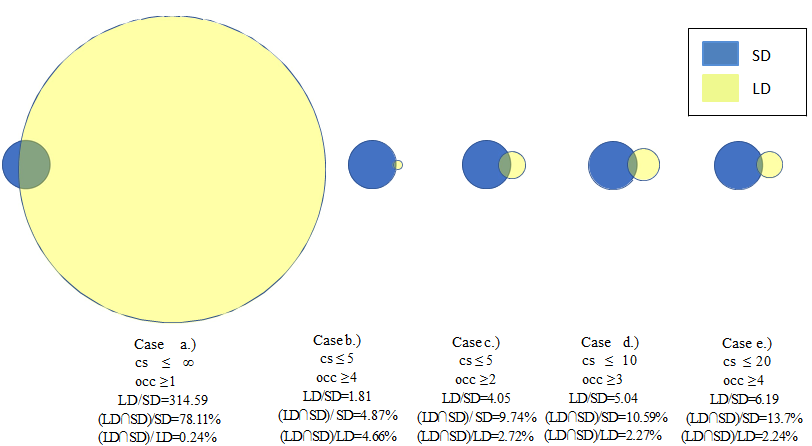
\includegraphics[width=6in]{figvennpdf.png}
% where an .eps filename suffix will be assumed under latex, 
% and a .pdf suffix will be assumed for pdflatex; or what has been declared
% via \DeclareGraphicsExtensions.
\caption{Intersections of logical and structural dependencies, in different cases defined by different combinations of filtering thresholds. }
\label{fig_venn}
\end{figure*}




\textit{\textbf{Question 2}}. Considering changes in comments only as valid can lead to additional logical dependencies? How many logical dependencies are introduced by considering comment changes as valid changes and in what percentage this can influence the analysis?

In order to assess the influence of comments, we compare pairwise subtables A. and B.,  subtables C. and D., and subtables E. and F. from table \ref{tab:perc}. We observe that the differences are not significant, the decrease represents  4\%-10\% of the value with comments, thus we can say that eliminating changes due only to comments can slightly improve the quality of finding logical dependencies.


\textit{\textbf{Question 3}}. How many occurrences of a logical dependency are needed to consider it a \textit{valid} logical dependency ? 

Based on the results presented in subtables E. and F. of table \ref{tab:perc}, we observe that we can obtain a number of logical dependencies which is between one quarter and one third of the number of the structural dependencies either by setting a commit size threshold of 5 files combined with an occurrence threshold of 2, or a commit size threshold of 10 files combined with an occurrence threshold of 3, or a commit size threshold of 20 files combined with an occurrence threshold of 4.  It is clear that increasing the threshold value for number of occurrences can be done only together with increasing the threshold value for maximum number of committed files. A more complex filtering condition can aggregate the 3 simple filtering cases, in the form: $((cs\leq 5) and (occ\geq 2)) or ((cs\leq 10) and (occ\geq 3)) or ((cs\leq 20) and (occ\geq 4))$. The filtering cases are presented in Figure \ref{fig_venn} cases b. and c. respectively d.

 
\section{Lessons learned and future work}

An issue which has not been investigated enough is whether the reduced set of logical dependencies obtained after filtering contains indeed true logical dependencies. This could be done by manual inspection of the classes in order to validate the logical dependencies by the opinion of a human expert. Unfortunately doing such manual validation is an impossibly huge task. We have manually inspected the code and code changes from a few of the case studies and the results seem promising. For example, in the case of the project selma, when filtering with both thresholds on commit size and number of occurrences, the tool reduced the initial set of 4751 co-change links identified between classes when no filtering was done, to a number of just 25 logical dependencies. Out of these 25 logical dependencies, 5 are doubled by structural dependencies. From the 20 remaining logical dependencies identified by the tool, we determined by manual inspection that 18 are logical, while for 2 of them we could not see a logical reason for a dependency relationship. 

We consider that in the future, the validation of extracted logical dependencies will occur by using them to enhance dependency graphs for applications such as architectural reconstruction \cite{Shtern:2012:CMS:2332427.2332428}, \cite{sar}  through clustering \cite{SoraConti} or finding of key classes \cite{PagerankENASE}, and evaluating the positive impact on their results.

As we could see in table \ref{tab:perc} C. and D., only a small amount of logical dependencies are between classes that also present structural dependencies.  In our experiments, even after filtering, around 80\% of the logical dependencies are between classes without structural dependencies. Although this big percentage is supported also by experiments of related works \cite{DBLP:journals/jss/AjienkaC17}, \cite{Oliva:2011:ISL:2067853.2068086}, we consider that future work must further investigate its cause. One possible cause could be that some of the co-changes were legit logical dependencies at some moment in the past, maybe even doubled by structural dependencies in previous revisions, but in the mean time the problem causing them may have been refactored and they should not be added to the dependency model of the current system.  

In this work we have extracted logical dependencies from all the revisions of the system, and structural dependencies from the last revision of the system. In future work we will take into account also structural dependencies from all the revisions of the system, in order to filter out the old, out-of-date logical dependencies. If we take into consideration also structural dependencies from previous revisions then the overlapping rate between logical and structural dependencies could probably increase. Another way to investigate this problem could be to study the trend of occurrences of co-changes: if co-changes between a pair of classes used to happen more often in the remote past than in the more recent past, it may be a sign that the problem causing the logical coupling has been removed in the mean time. 


\section{Conclusion}
\label{sec:Conclusion}
   
In this work we experimentally define methods to filter out the most relevant logical dependencies from co-changing classes. 

Our experiments showed that the most important factors studied until now, which affect the quality of logical dependencies are: the maximum number of files allowed in a commit to be counted as logical dependency, and the minimum number of repeated occurrences for a co-change to be counted as logical dependency. Increasing the threshold value for the number of occurrences can be done only together with increasing the threshold value for the maximum number of files allowed in a commit.

We have identified also new factors such as the history of structural dependencies and the trend of co-change occurrences which will be investigated in future work.The validation of our method for identifying logical dependencies will come by measuring the impact of using them to enhance dependency models used in applications of architectural reconstruction.


% conference papers do not normally have an appendix


% use section* for acknowledgment
%\section*{Acknowledgment}
%
%This work was partially supported by a grant of the Romanian National Authority for Scientific Research and Innovation, CNCS/CCCDI UEFISCDI, project number PN-III-P2-2.1-PED-2016-0999, within PNCDI III.


% trigger a \newpage just before the given reference
% number - used to balance the columns on the last page
% adjust value as needed - may need to be readjusted if
% the document is modified later
%\IEEEtriggeratref{8}
% The "triggered" command can be changed if desired:
%\IEEEtriggercmd{\enlargethispage{-5in}}

% references section

% can use a bibliography generated by BibTeX as a .bbl file
% BibTeX documentation can be easily obtained at:
% http://mirror.ctan.org/biblio/bibtex/contrib/doc/
% The IEEEtran BibTeX style support page is at:
% http://www.michaelshell.org/tex/ieeetran/bibtex/
\bibliographystyle{IEEEtran}
% argument is your BibTeX string definitions and bibliography database(s)
\bibliography{IEEEabrv,logicaldepd}
%
% <OR> manually copy in the resultant .bbl file
% set second argument of \begin to the number of references
% (used to reserve space for the reference number labels box)
%\begin{thebibliography}{1}
%
%\bibitem{IEEEhowto:kopka}
%H.~Kopka and P.~W. Daly, \emph{A Guide to \LaTeX}, 3rd~ed.\hskip 1em plus
% 0.5em minus 0.4em\relax Harlow, England: Addison-Wesley, 1999.
%
%\end{thebibliography}




% that's all folks
\end{document}


